\section*{Problem 2}
Consider the 3-noded isoparametric quadratic element shown in Fig.

\begin{figure}[h!]
    \centering
    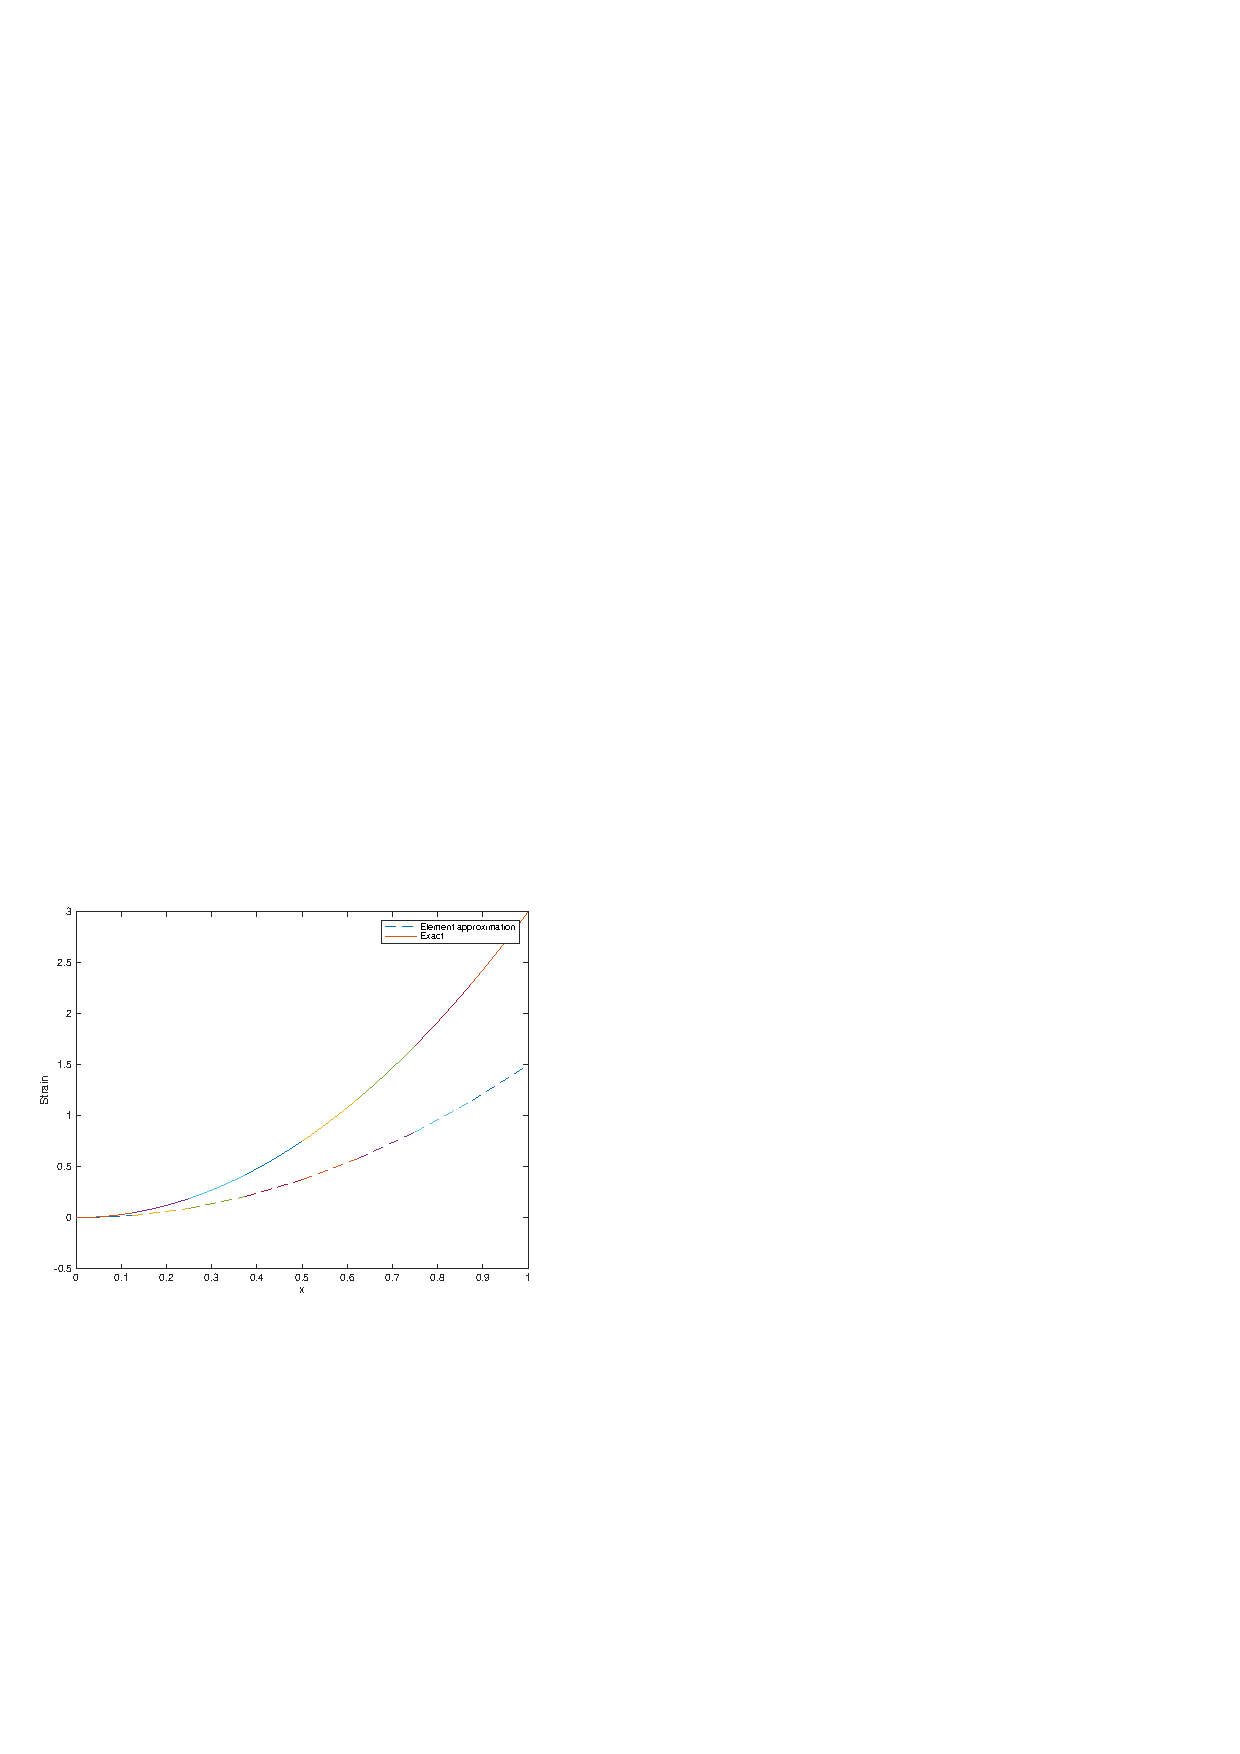
\includegraphics[width=0.5\textwidth]{figure_1.png}  % Replace with your image file name
    \caption{Problem 1}
    \label{fig:element}
\end{figure}

\begin{enumerate}
    \item[(a)] \textbf{(20 points)} Verify that if the nodes are uniformly spaced, the element Jacobian is given by \( J = \frac{L}{2} \).

    
    \item[(b)] \textbf{(20 points)} If \( \epsilon_x \) at node 1 is to remain finite, how far from the center can node 2 be moved?
 
\end{enumerate}


\subsection*{a.$)$}
 Verify that if the nodes are uniformly spaced, the element Jacobian is given by $J = \frac{L}{2}$

Note: I did most all of the math and calculated these values when I was trying to solve problem 1. I worked on the problems in order, and did not know that I would be calcuating the values that I used in problem 1 later. So in this section I restate the results and what
I did to get the values, because the math is calculated in problem 1.

\subsubsection*{Step 1: Define the Coordinates and the Mapping}
For a three-node isoparametric quadratic element with nodes located at \(\xi = -1\), \(\xi = 0\), and \(\xi = 1\), the global coordinates \( x \) at any point within the element can be expressed in terms of the shape functions and nodal coordinates \( x_1 \), \( x_2 \), and \( x_3 \) as:

\[
x(\xi) = N_1(\xi) x_1 + N_2(\xi) x_2 + N_3(\xi) x_3,
\]

where:
\begin{itemize}
    \item \( N_1(\xi) = \frac{1}{2} \xi (\xi - 1) \),
    \item \( N_2(\xi) = 1 - \xi^2 \),
    \item \( N_3(\xi) = \frac{1}{2} \xi (\xi + 1) \).
\end{itemize}

\subsubsection*{Step 2: Substitute Uniform Node Spacing}
Assume that the nodes are uniformly spaced along the length \( L \) of the element:
\begin{align*}
    x_1 &= -\frac{L}{2}, \\
    x_2 &= 0, \\
    x_3 &= \frac{L}{2}.
\end{align*}

\subsubsection*{Step 3: Calculate the Jacobian \( J = \frac{dx}{d\xi} \)}
The Jacobian \( J \) is defined as the derivative of \( x \) with respect to \( \xi \):

\[
J = \frac{dx}{d\xi}.
\]

Using the expression for \( x(\xi) \), we differentiate with respect to \( \xi \):

\[
\frac{dx}{d\xi} = \frac{dN_1}{d\xi} x_1 + \frac{dN_2}{d\xi} x_2 + \frac{dN_3}{d\xi} x_3.
\]

\subsubsection*{Step 4: Calculate Each Derivative of the Shape Functions}
Now, calculate \( \frac{dN_1}{d\xi} \), \( \frac{dN_2}{d\xi} \), and \( \frac{dN_3}{d\xi} \):

1. For \( N_1(\xi) = \frac{1}{2} \xi (\xi - 1) \):
   \[
   \frac{dN_1}{d\xi} = \frac{1}{2} (2\xi - 1) = \xi - \frac{1}{2}.
   \]

2. For \( N_2(\xi) = 1 - \xi^2 \):
   \[
   \frac{dN_2}{d\xi} = -2\xi.
   \]

3. For \( N_3(\xi) = \frac{1}{2} \xi (\xi + 1) \):
   \[
   \frac{dN_3}{d\xi} = \frac{1}{2} (2\xi + 1) = \xi + \frac{1}{2}.
   \]

\subsubsection*{Step 5: Substitute and Simplify}
Substitute these derivatives and the values of \( x_1 \), \( x_2 \), and \( x_3 \) into the Jacobian expression:

\[
J = \frac{dx}{d\xi} = \left(\xi - \frac{1}{2}\right) \left(-\frac{L}{2}\right) + (-2\xi) \cdot 0 + \left(\xi + \frac{1}{2}\right) \frac{L}{2}.
\]

Simplifying, we get:

\[
J = -\frac{L}{2} \left(\xi - \frac{1}{2}\right) + \frac{L}{2} \left(\xi + \frac{1}{2}\right).
\]

Expanding both terms:

\[
J = -\frac{L}{2} \xi + \frac{L}{4} + \frac{L}{2} \xi + \frac{L}{4}.
\]

Combine terms:

\[
J = \frac{L}{2}.
\]

\subsubsection*{Conclusion}
Thus, we have verified that the Jacobian for this uniformly spaced three-node isoparametric quadratic element is indeed \( J = \frac{L}{2} \), as required.

\subsection*{b.$)$}
If \( \epsilon_x \) at node 1 is to remain finite, how far from the center can node 2 be moved?


\subsubsection*{1. Displacement Field and Strain for a Quadratic Element}
I did this in problem 1 too, so I will just quickly restate the values that I calculated from that problem.\\

For a three-node isoparametric quadratic element, the displacement field \( u(x) \) in terms of the natural coordinate \( \xi \) and nodal displacements \( u_1 \), \( u_2 \), and \( u_3 \) is:

\[
u(\xi) = N_1(\xi) u_1 + N_2(\xi) u_2 + N_3(\xi) u_3,
\]

where:
- \( N_1(\xi) = \frac{1}{2} \xi (\xi - 1) \),
- \( N_2(\xi) = 1 - \xi^2 \),
- \( N_3(\xi) = \frac{1}{2} \xi (\xi + 1) \).

The strain \( \epsilon_x \) is the derivative of the displacement with respect to \( x \):

\[
\epsilon_x = \frac{du}{dx}.
\]

Since we are working in terms of \( \xi \), we use the chain rule:

\[
\epsilon_x = \frac{du}{d\xi} \cdot \frac{d\xi}{dx}.
\]

\subsubsection*{2. Derivative of \( u \) with Respect to \( \xi \)}

Taking the derivative of \( u(\xi) \) with respect to \( \xi \):

\[
\frac{du}{d\xi} = \frac{dN_1}{d\xi} u_1 + \frac{dN_2}{d\xi} u_2 + \frac{dN_3}{d\xi} u_3.
\]

Using the derivatives of the shape functions:
- \( \frac{dN_1}{d\xi} = \xi - \frac{1}{2} \),
- \( \frac{dN_2}{d\xi} = -2\xi \),
- \( \frac{dN_3}{d\xi} = \xi + \frac{1}{2} \),

we can write:

\[
\frac{du}{d\xi} = \left( \xi - \frac{1}{2} \right) u_1 - 2\xi u_2 + \left( \xi + \frac{1}{2} \right) u_3.
\]

\subsubsection*{3. Jacobian \( \frac{d\xi}{dx} \)}

The Jacobian \( J = \frac{dx}{d\xi} \) for this element maps between the natural coordinate \( \xi \) and the physical coordinate \( x \):

\[
\frac{dx}{d\xi} = \frac{dN_1}{d\xi} x_1 + \frac{dN_2}{d\xi} x_2 + \frac{dN_3}{d\xi} x_3.
\]

Substituting \( x_1 \), \( x_2 \), and \( x_3 \), and using the derivatives of the shape functions, we get:

\[
\frac{dx}{d\xi} = \left( \xi - \frac{1}{2} \right) x_1 - 2\xi x_2 + \left( \xi + \frac{1}{2} \right) x_3.
\]

The strain \( \epsilon_x \) becomes:

\[
\epsilon_x = \frac{du}{d\xi} \cdot \frac{1}{\frac{dx}{d\xi}}.
\]

\subsubsection*{4. Behavior of \( \frac{dx}{d\xi} \) as Node 2 Approaches Node 1 or Node 3}

1. If node 2 approaches node 1:\\
   - As \( x_2 \) approaches \( x_1 \), the distance between nodes 1 and 2 shrinks.\\
   - In this case, the terms involving \( x_1 \) and \( x_2 \) in \( \frac{dx}{d\xi} \) nearly cancel each other out, making \( \frac{dx}{d\xi} \) very small.\\
   - Since \( \epsilon_x = \frac{du}{d\xi} \cdot \frac{1}{\frac{dx}{d\xi}} \), a small \( \frac{dx}{d\xi} \) in the denominator causes \( \epsilon_x \) to become very large.\\

2. If node 2 approaches node 3:\\
   - Similarly, as \( x_2 \) approaches \( x_3 \), the distance between nodes 2 and 3 shrinks.\\
   - This causes the terms involving \( x_2 \) and \( x_3 \) in \( \frac{dx}{d\xi} \) to nearly cancel out, again making \( \frac{dx}{d\xi} \) very small.\\
   - With \( \frac{dx}{d\xi} \) small, the strain \( \epsilon_x \) again becomes large due to division by a small number.\\

\subsubsection*{Conclusion}

To keep \( \epsilon_x \) finite, node 2 must stay far from nodes 1 and 3 to avoid \( \frac{dx}{d\xi} \) approaching zero. Moving node 2 too close to either node 1 or node 3 leads to strain approaching infinity. 
So, node 2 should remain within a certain range around the center for the strain to remain finite.

The distance \( x_2 \) from the center should remain within \( -\frac{L}{2} < x_2 < \frac{L}{2} \), with \( x_2 \) ideally not too close to either boundary.
